\section{Results and evaluation} \label{sec:results}

\subsection{Evaluating distance metric}

To evaluate our implementation of the $k$-mer distance using windows and the
Jaccard index, the Levenshtein distance was used as reference. Since the
Levenshtein distance does not produce values between $0$ and $1$, the Jaccard
index was used here as well.

In figure \ref{fig:Levenshtein_vs_Kmer} is three scatter plots with the
Levenshtein distance on the $y$-axis and our version of the $k$-mer distance on
the $x$-axis. The three plots are with $k=4, k=6$ and $k=8$.

The scatter plots gives an indication about when and how sensitive our
implemented distance metric is. We want the distance to be as close as possible
to a linear function without too much variance, but not necessarily to the line
$y=x$. If it can be expressed linearly it means there is a correlation between
the two. If it can be expressed as $y=x$ (or close) it means that they measure
the same distance which is favourable.

When $k=4$ there is a linear relation when the identity $I>0.9$, but when
$I<0.9$ there is too much variance in the points from any linear function.

With $k=6$ there seems to be a linear relation when $I>0.8$. When $I<0.8$ there
is more variance though less than when $k=4$.

When $k=8$, it is very similar to $k=6$. It seems there is a linear relation
for $I>0.8$ again and when $I<0.8$ the variance is greater.

\begin{figure}
  \begin{subfigure}[b]{0.5\textwidth}
    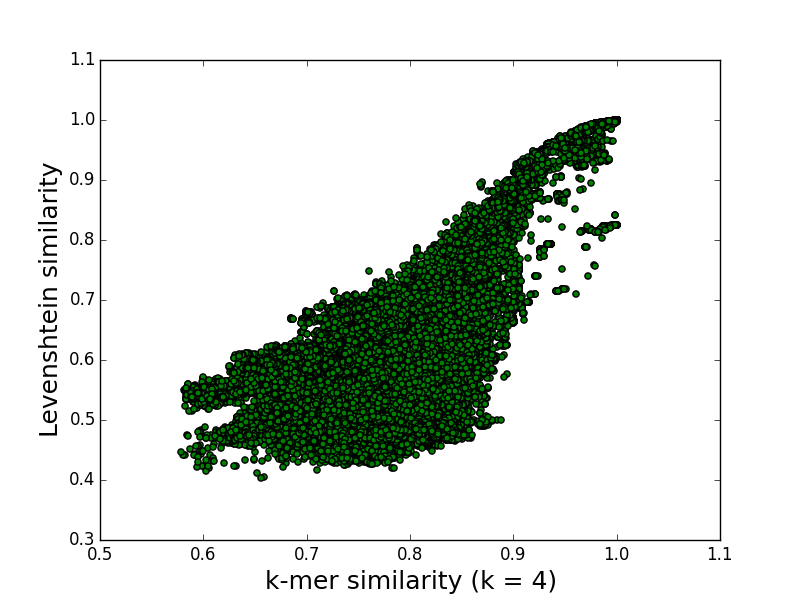
\includegraphics[scale=0.34]{graphics/k4.png}
  \end{subfigure}
  \begin{subfigure}[b]{0.5\textwidth}
    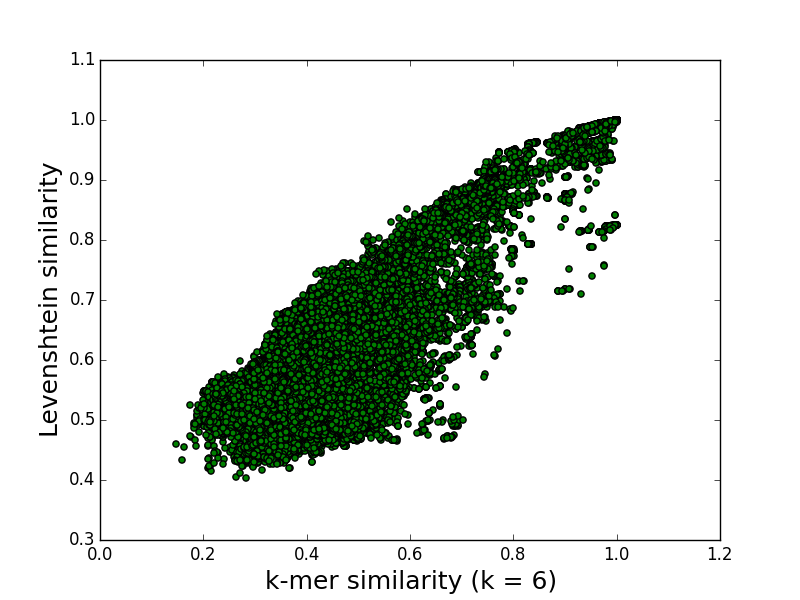
\includegraphics[scale=0.34]{graphics/k6.png}
  \end{subfigure}

  \centering
  \begin{subfigure}[b]{0.5\textwidth}
    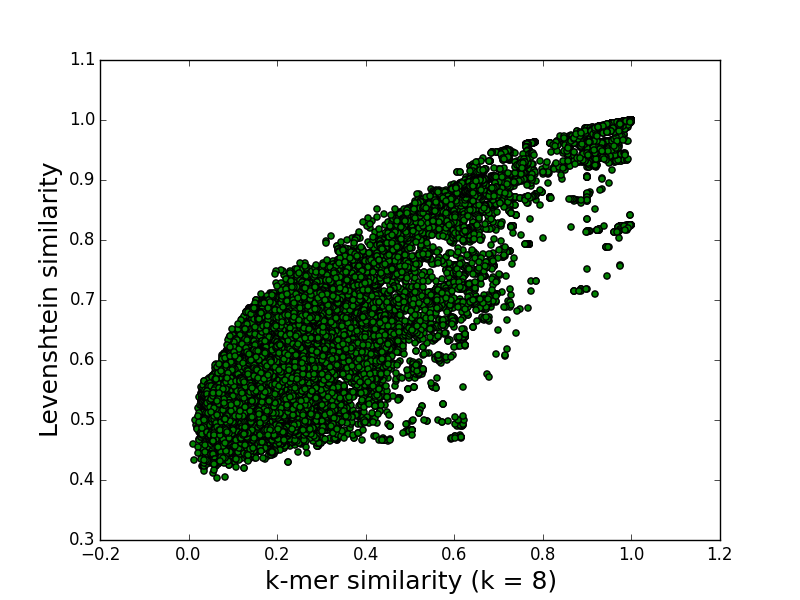
\includegraphics[scale=0.34]{graphics/k8.png}
  \end{subfigure}
  \caption{Comparison of Levenshtein distance and our implementation of the
  $k$-mer distance using windows and Jaccard index.}
  \label{fig:Levenshtein_vs_Kmer}
\end{figure}


\subsection{Comparing with UCLUST on real life data}
% Testing USEARCH 32-bit on real data
% Testing clustering algorithm with d2 distance and comparing performance to
% USEARCH.
Running \texttt{USEARCH} on the file
\texttt{SILVA\_119\_SSURef\_tax\_silva.fasta} after it is sorted with
parameters \texttt{-clust\_smallmem} and \texttt{-id 0.95} produces the
following output

\begin{lstlisting}[style=output-style,
  caption=Output from \texttt{USEARCH} clustering.,
  label=fig:uclust_silva]
28:39 1.1Gb  100.0\% 117205 clusters, max size 83904, avg 13.5
      Seqs  1583830 (1.6M)
  Clusters  117205 (117.2k)
  Max size  83904 (83.9k)
  Avg size  13.5
  Min size  1
Singletons  67410 (67.4k), 4.3\% of seqs, 57.5\% of clusters
   Max mem  1.1Gb
      Time  28:41
Throughput  920.3 seqs/sec.
\end{lstlisting}

Running our implementation of the same file but unsorted and with
\texttt{id=0.9, k=6} og \texttt{max\_rejects=8} produces the following

\begin{lstlisting}[style=output-style]
Reading 1583830 sequences...
Finished reading:
Time: 24.8109 sec.
Seqs/sec: 63836
Clustering 1583830 sequences...
26.4602
# of clusters: 1364006
Finished clustering:
Time: 187.355 sec.
Throughput: 8453.63seqs/sec.
\end{lstlisting}

Even though the \texttt{id}'s does not represent the same threshold due to it
being two different distance metrics we do get a lot more clusters. Running
it with similar \texttt{id}'s produces almost the same amount of clusters, so
the problem lies in the way we choose our centroids we compare a query
sequence with.

Our implementation, however, is faster by a factor of $10$. This can be
attributed to our choice of distance metric.

%Possibly things to look into: confusion matrix, Rand index, normalized
%mutual information (article: Comparing Clusterings - An Overview).


\subsection{Results}
\begin{figure}[H]
  \centering
  \begin{tabular}{ c | c }
    Metric                                        & Comparisons/second      \\
    \hline \hline
    Dynamic programming (bottom up) Levenshtein   & $\sim$ 70               \\
    \hline
    d2-distance with window, $k=4$                & $\sim$ 73000            \\
    \hline
    d2-distance with window, $k=6$                & $\sim$ 63000            \\
    \hline
    d2-distance with window, $k=8$                & $\sim$ 24000            \\
  \end{tabular}
  \caption{Performance of different distance metrics.}
\end{figure}

\begin{figure}[H]
  \centering
  \begin{tabular}{ p{12em} | c | c }
    Method  & Throughput/second   & \# of clusters \\
    \hline \hline
    \textsc{Simple\_Clust}, $k=4$,
    $max\_rejects=8$, $id=0.97$     & $\sim$ 11,400  & 444,654  \\
    \hline
    \textsc{Simple\_Clust}, $k=5$,
    $max\_rejects=8$, $id=0.97$     & $\sim$ 10,700  & 461,266  \\
    \hline
    \textsc{Simple\_Clust}, $k=6$,
    $max\_rejects=8$, $id=0.97$     & $\sim$ 9,575   & 470,516  \\
    \hline
    \textsc{Simple\_Clust}, $k=7$,
    $max\_rejects=8$, $id=0.97$     & $\sim$ 6,350   & 474,463  \\
    \hline
    \textsc{Simple\_Clust}, $k=8$,
    $max\_rejects=8$, $id=0.97$     & $\sim$ 2,750   & 475,465  \\
  \end{tabular}
  \caption{Performance of different clustering methods and different $k$-mer
  sizes. Sequence data:
           \texttt{RDP\_Pro\_Full\_sort.fna}. Count: 500,000. Throughput
           specifies the number of sequences clustered per second (including
           results output to file), but excludes reading the input file.}
\end{figure}
